Firebase es una plataforma de desarrollo de aplicaciones móviles y web que
ofrece una variedad de herramientas y servicios en la nube para ayudar a los
desarrolladores a crear, mejorar y escalar aplicaciones.
\begin{figure}[htb!]
    \centering
    \caption{Logo de Firebase}
    \label{fig:firebase-logo}
    \centering
    
\includegraphics[scale=0.35]{./Ilustraciones/logos/Firebase.png}\\
    \textbf{Fuente:} Página oficial de Firebase [\url{https://firebase.google.com/?hl=es}]
\end{figure}
\hfill \break
Firebase fue adquirido por Google en 2014 y desde entonces ha evolucionado para
ofrecer una amplia gama de servicios, incluyendo:
\begin{itemize}
    \item Autenticación de usuarios[Capítulo \ref{autenticacion}]: permite a los
          desarrolladores agregar fácilmente funciones de registro, inicio de sesión y
          autenticación a sus aplicaciones.
    \item Almacenamiento en la nube[Capítulo \ref{almacenamiento}]: proporciona
          almacenamiento en la nube para archivos y datos de aplicaciones.
    \item Base de datos en tiempo real: una base de datos en tiempo real en la nube que
          permite a los desarrolladores crear aplicaciones en tiempo real con
          actualizaciones automáticas y en tiempo real.
    \item Alojamiento de aplicaciones web: permite a los desarrolladores alojar sus
          aplicaciones web en los servidores de Firebase.
    \item Notificaciones push: permite enviar notificaciones push a los usuarios de la
          aplicación.
    \item Analítica de aplicaciones: proporciona análisis de usuarios y datos de uso de
          la aplicación.
\end{itemize}

Para este proyecto no se ha hecho uso de todas las utilidades, solamente de:

\subsubsection{Autenticación de usuarios}
\label{autenticacion} Se ha hecho uso de esta
utilidad debido a que nos proporciona una forma sencilla de registrar usuarios,
hacer que estos inicien sesión, y que puedan cerrar sesión de una forma simple.
Además, y como veremos en las conclusiones y trabajo futuro [Capítulo \ref{trabajo-futuro}],
nos permite hacer uso de la autenticación de Google, lo que nos permite tener
una mayor seguridad en el inicio de sesión de los usuarios.
\begin{figure}[htb!]
    \centering
    \caption{Tabla de autenticación proporcionada por Firebase}
    \label{fig:firebase-autenticacion}
    \centering
    \includegraphics[scale=0.65]{./Ilustraciones/autenticación.png}\\
    \textbf{Fuente:} Consola de Firebase, apartado de Autenticación
\end{figure}
\hfill \break

\subsubsection{Almacenamiento en la nube}
\label{almacenamiento}
Se ha hecho uso de esta utilidad debido a que nos proporciona una base de datos
en la nube, lo que nos permite tener una mayor seguridad en el almacenamiento de
los datos de los usuarios, y de la aplicación en general.
En este caso, guardamos 3 tipos de datos:
\begin{itemize}
    \item Los \textbf{usuarios} registrados, con la información del correo, si es
          administrador, el nombre, el apellido, su número de móvil, su nombre de
          usuario, que está compuesto por el inicio del correo y su primer nombre, y las
          carteras que este ha agregado.
    \item Las \textbf{colecciones} que se mostrarán de NFT's, que contienen las
          direcciones de las colecciones para poder acceder a las mismas, la url de la
          colleción, el nombre real y la foto de la marca.
    \item También se ha hecho un apartado para \textbf{mensajes}, el cual contiene
          mensajes qeu hand ejado los usuarios con intenciones de mejora. Este documento
          contiene el correo del usuario que lo ha mandado, el mensaje, y un asunto.
\end{itemize}

\begin{figure}[htb!]
    \centering
    \caption{Conjunto de colecciones y documentos proporcionada por Firebase}
    \label{fig:firebase-almacenamiento}
    \centering
    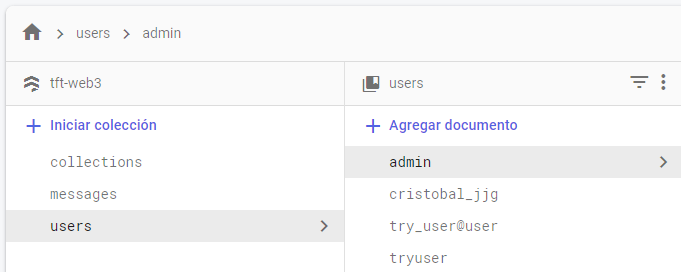
\includegraphics[scale=0.75]{./Ilustraciones/almacenamiento.png}\\
    \textbf{Fuente:} Consola de Firebase, apartado de Firestore Database
\end{figure}